\subsection{Pipelined Design}
So what is the purpose of a Pipelined version of a CPU\@? As stated in the previous section, the unpipelined version is quite slow since it needs to wait for the instruction to be executed before loading the next one. 
Pipelining follows the idea of dividing the work among smaller parts and executing them in parallel. In the case of a CPU, it means that we will divide the execution of an instruction into multiple stages and execute multiple instructions at the same time.
Since each part has a smaller quantity of work to do, we can hopefully increase the clock frequency and thus obtaining in average a better throughput resulting in better performance.

\begin{figure}[H]
    \centering
    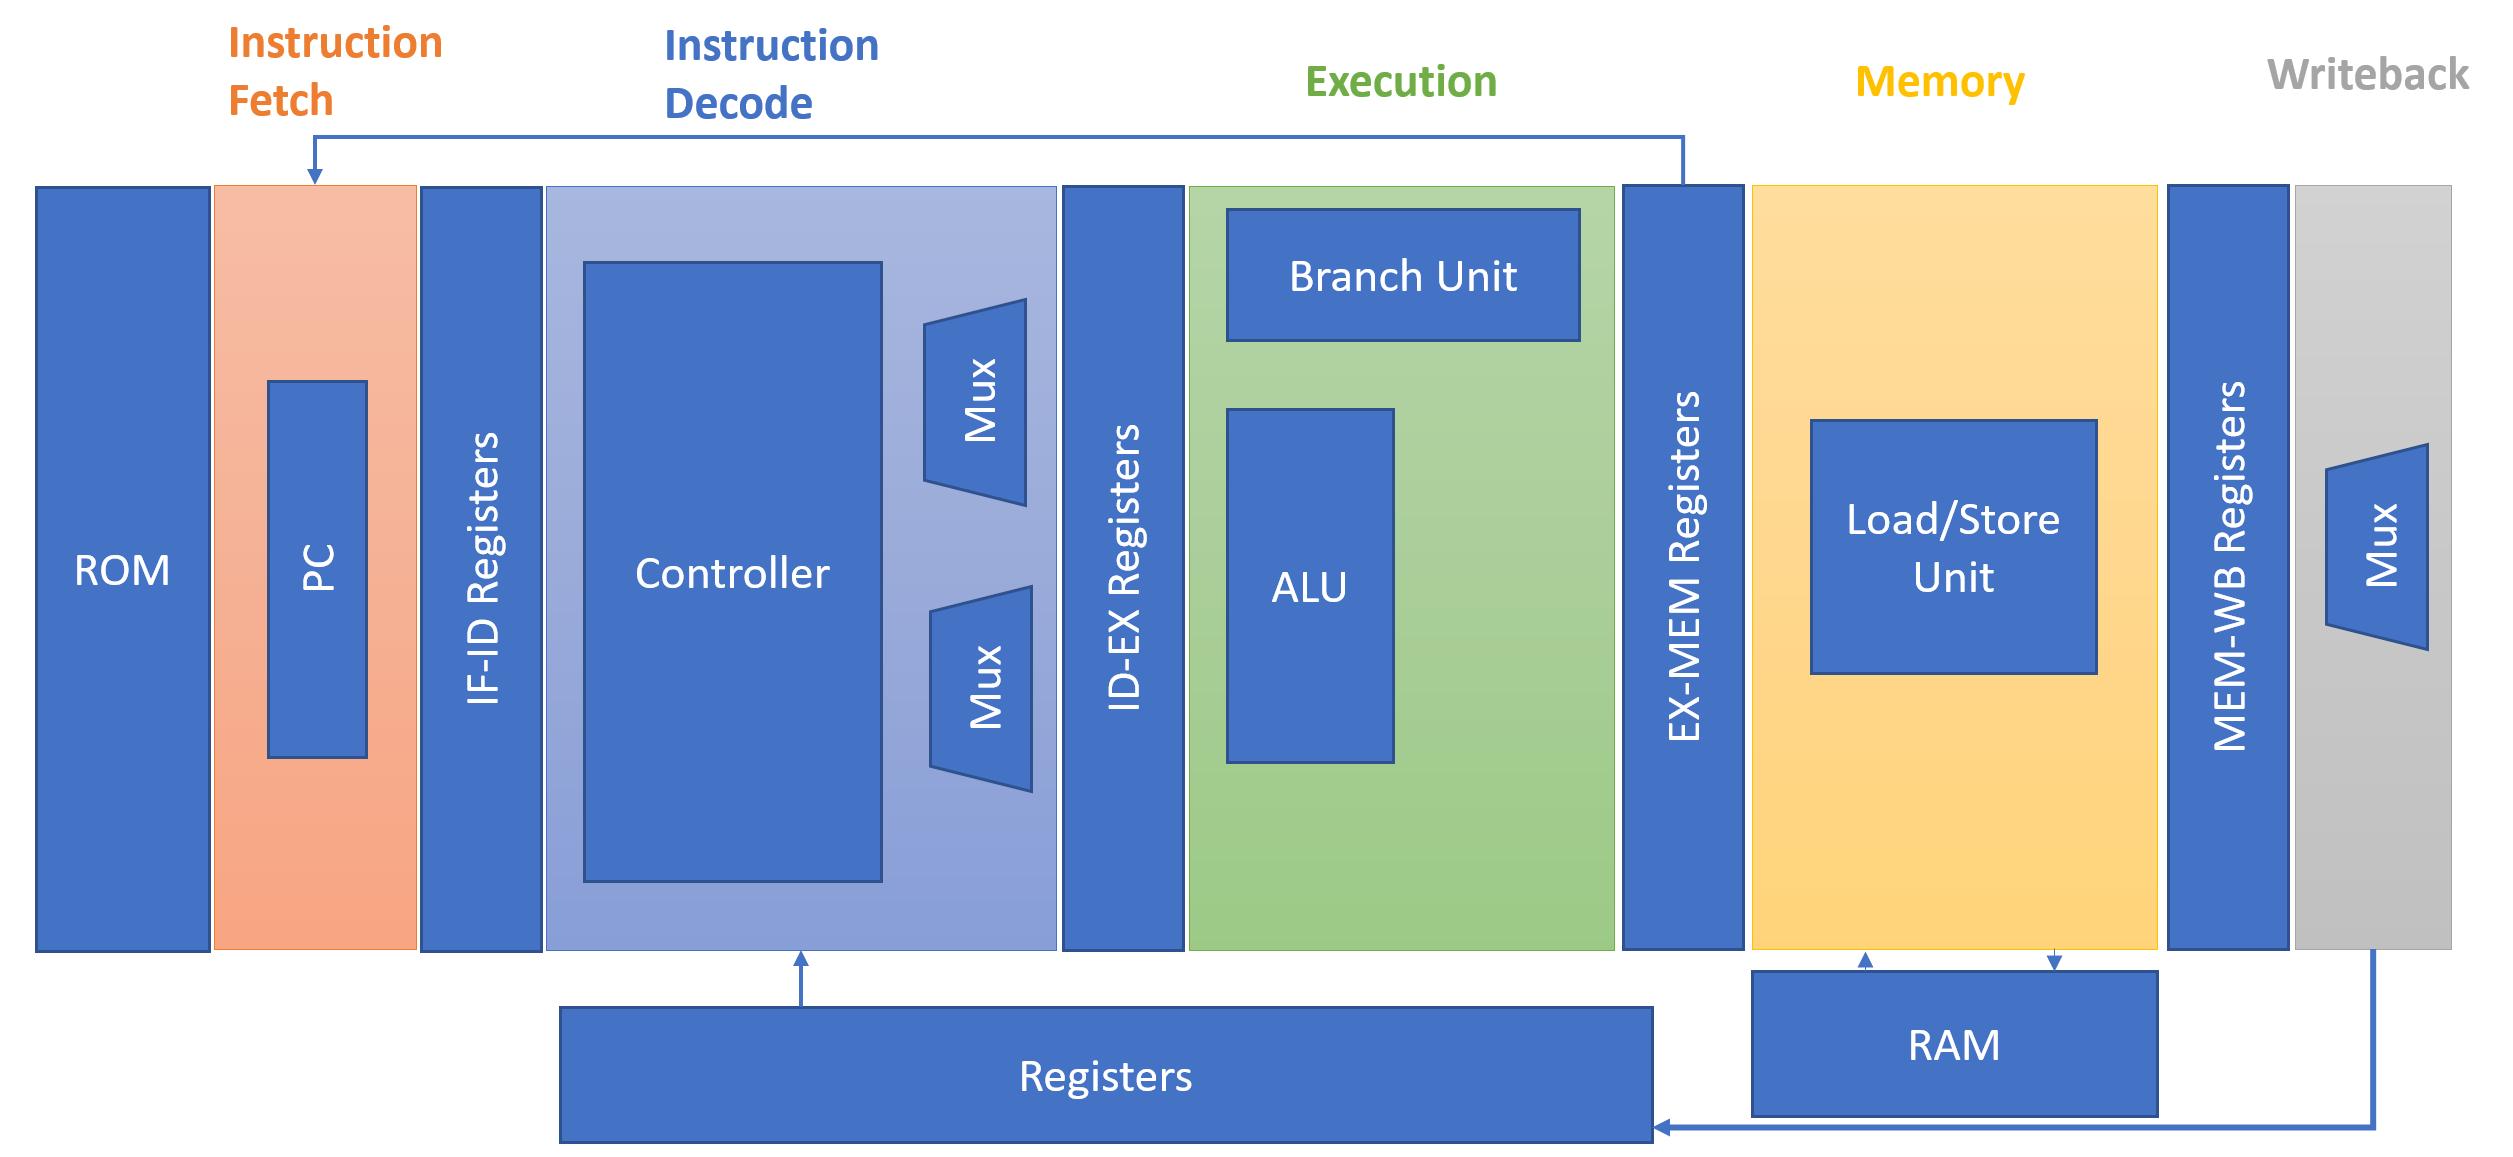
\includegraphics[width=1\textwidth]{design/pipelined/images/pipelined_design.png}
    \caption{Pipelined CPU design}
    \label{fig:pipelined_cpu_design}
\end{figure}

So here is the idea, we will divide the execution of instruction into five stages: Instruction Fetch (IF), Instruction Decode (ID), Execute (EX), Memory (MEM) and Write Back (WB).
Each stage will be executed in parallel and will be connected to the next one using pipeline registers. The pipeline registers are used to store the data between each stage and are synchronized with the clock.
The IF stage will fetch the instruction from the ROM using the PC (Program Counter) and will send it to the ID stage. The ID stage will decode the instruction and send the control signals to the different units 
(ALU, Branch Unit, Load/Store Unit) and will also send the operands to the EX stage. The EX stage will execute the instruction and send the result to the MEM stage. 
The MEM stage will load or store data from or to the RAM and send the result to the WB stage. Finally, the WB stage will write the result to the register file. \\

But for the most attentive reader or anybody with a bit of experience in computer architecture, you may have noticed that there is a problem with this design. 
This design will lead so some issues in two different ways. 

\begin{enumerate}[label=\textbullet]
    \item The first one is that since instruction is not executed anymore in one cycle, its result will not be available in the next cycle.
    This is an issue because if the next instruction depends on the result of the previous one, it will not be able to execute correctly and will use 
    outdated data from the registers. This is called a \textbf{Data Hazard}.
    \item The second one is related to the branching mechanism, since the result of the branch will be available only after the EX stage, the PC will not be updated
    before that leading to possible wrong instructions being fetched and executed in the pipeline. This is called a \textbf{Control Hazard}.
\end{enumerate}

For resolving these two issues we have two solutions. Either stalling the pipeline when a hazard is occurring or when a branch is detected at the IF stage such that we wait for 
the result before fetching any new instruction. One issue with this approach is of course performance which is unfortunate since the main purpose of pipelining is to improve performance.

Another solution for the data hazard is to use \textbf{Forwarding} which consists of forwarding the result of the ALU to the EX stage and the result of the MEM stage to the EX and MEM stages.
The only moment we will have to stall the pipeline is when we have a load instruction followed by an instruction using the result of the load. In this case, we will have to stall the pipeline
for one cycle to wait for the result of the load.

\begin{figure}[H]
    \centering
    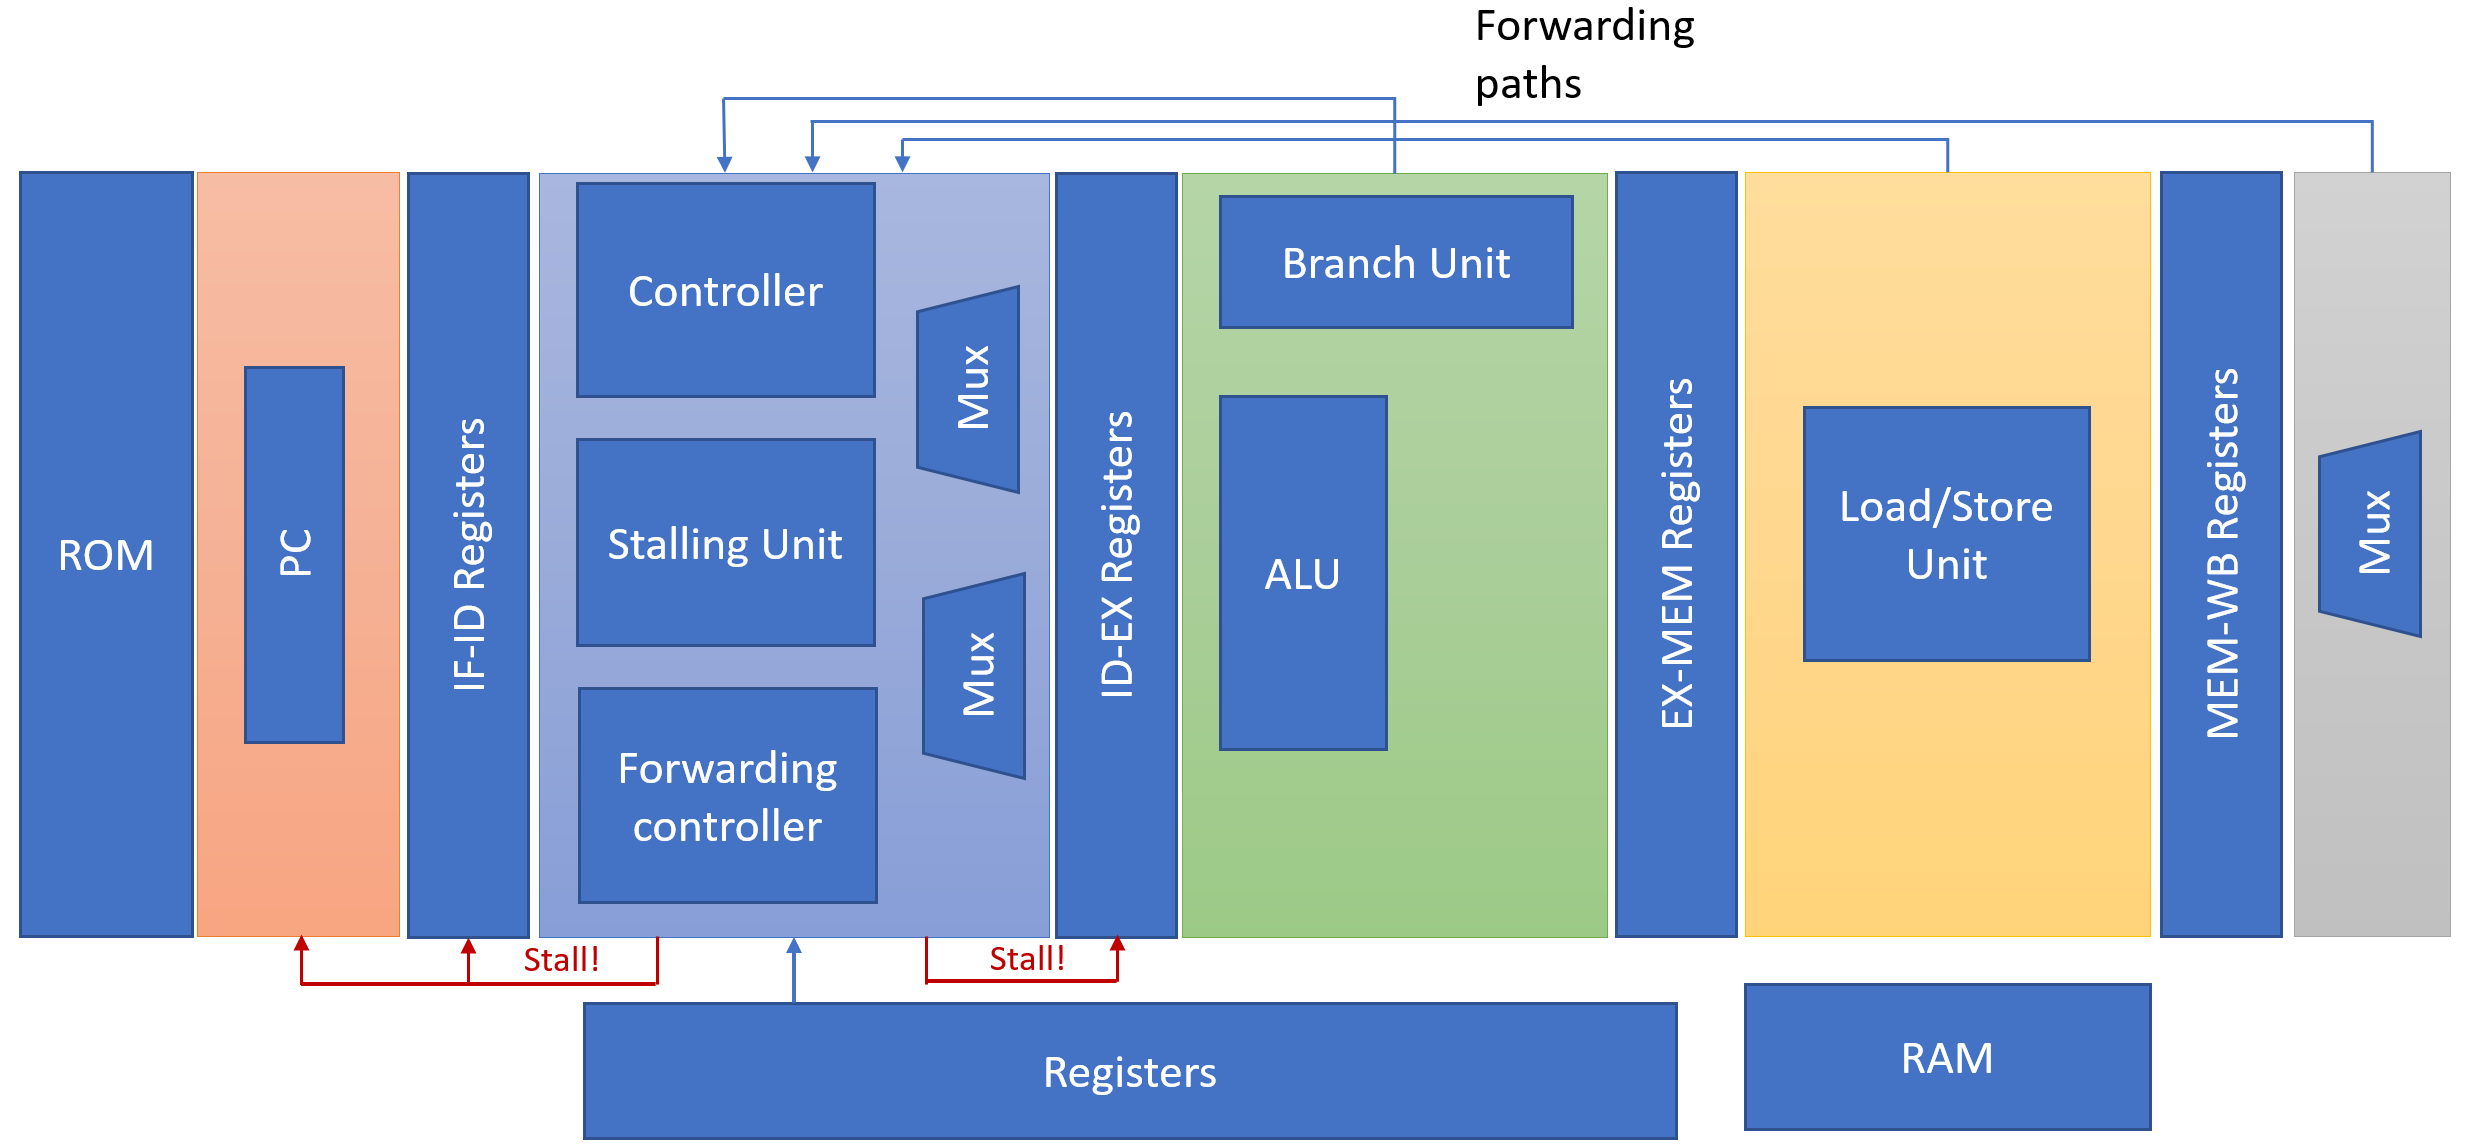
\includegraphics[width=1\textwidth]{design/pipelined/images/pipelined_design_forwarding.png}
    \caption{Pipelined CPU design with forwarding paths}
    \label{fig:pipelined_cpu_design_forwarding}
\end{figure}

Another solution for the control hazard is to use \textbf{Branch Prediction} which consists of predicting the result of the branch and fetching the instruction at the predicted address.
It is not always possible to predict correctly the result of a branch but it is possible to use some heuristics to improve the prediction accuracy. For example, we can predict that a branch will not be taken
if the previous branch was not taken. This is called a \textbf{Branch Not Taken} heuristic. Another heuristic is to predict that a branch will be taken if the previous branch was taken. This is called a \textbf{Branch Taken} heuristic.
Of course, you can develop more complex heuristics but this is out of the scope of this project and I invite you to use the link in the reference to the given algorithm I've chosen 
to implement in the CPU\@. But when the prediction is wrong, we will have to flush the pipeline and restart the execution from the correct address. \\

\begin{figure}[H]
    \centering
    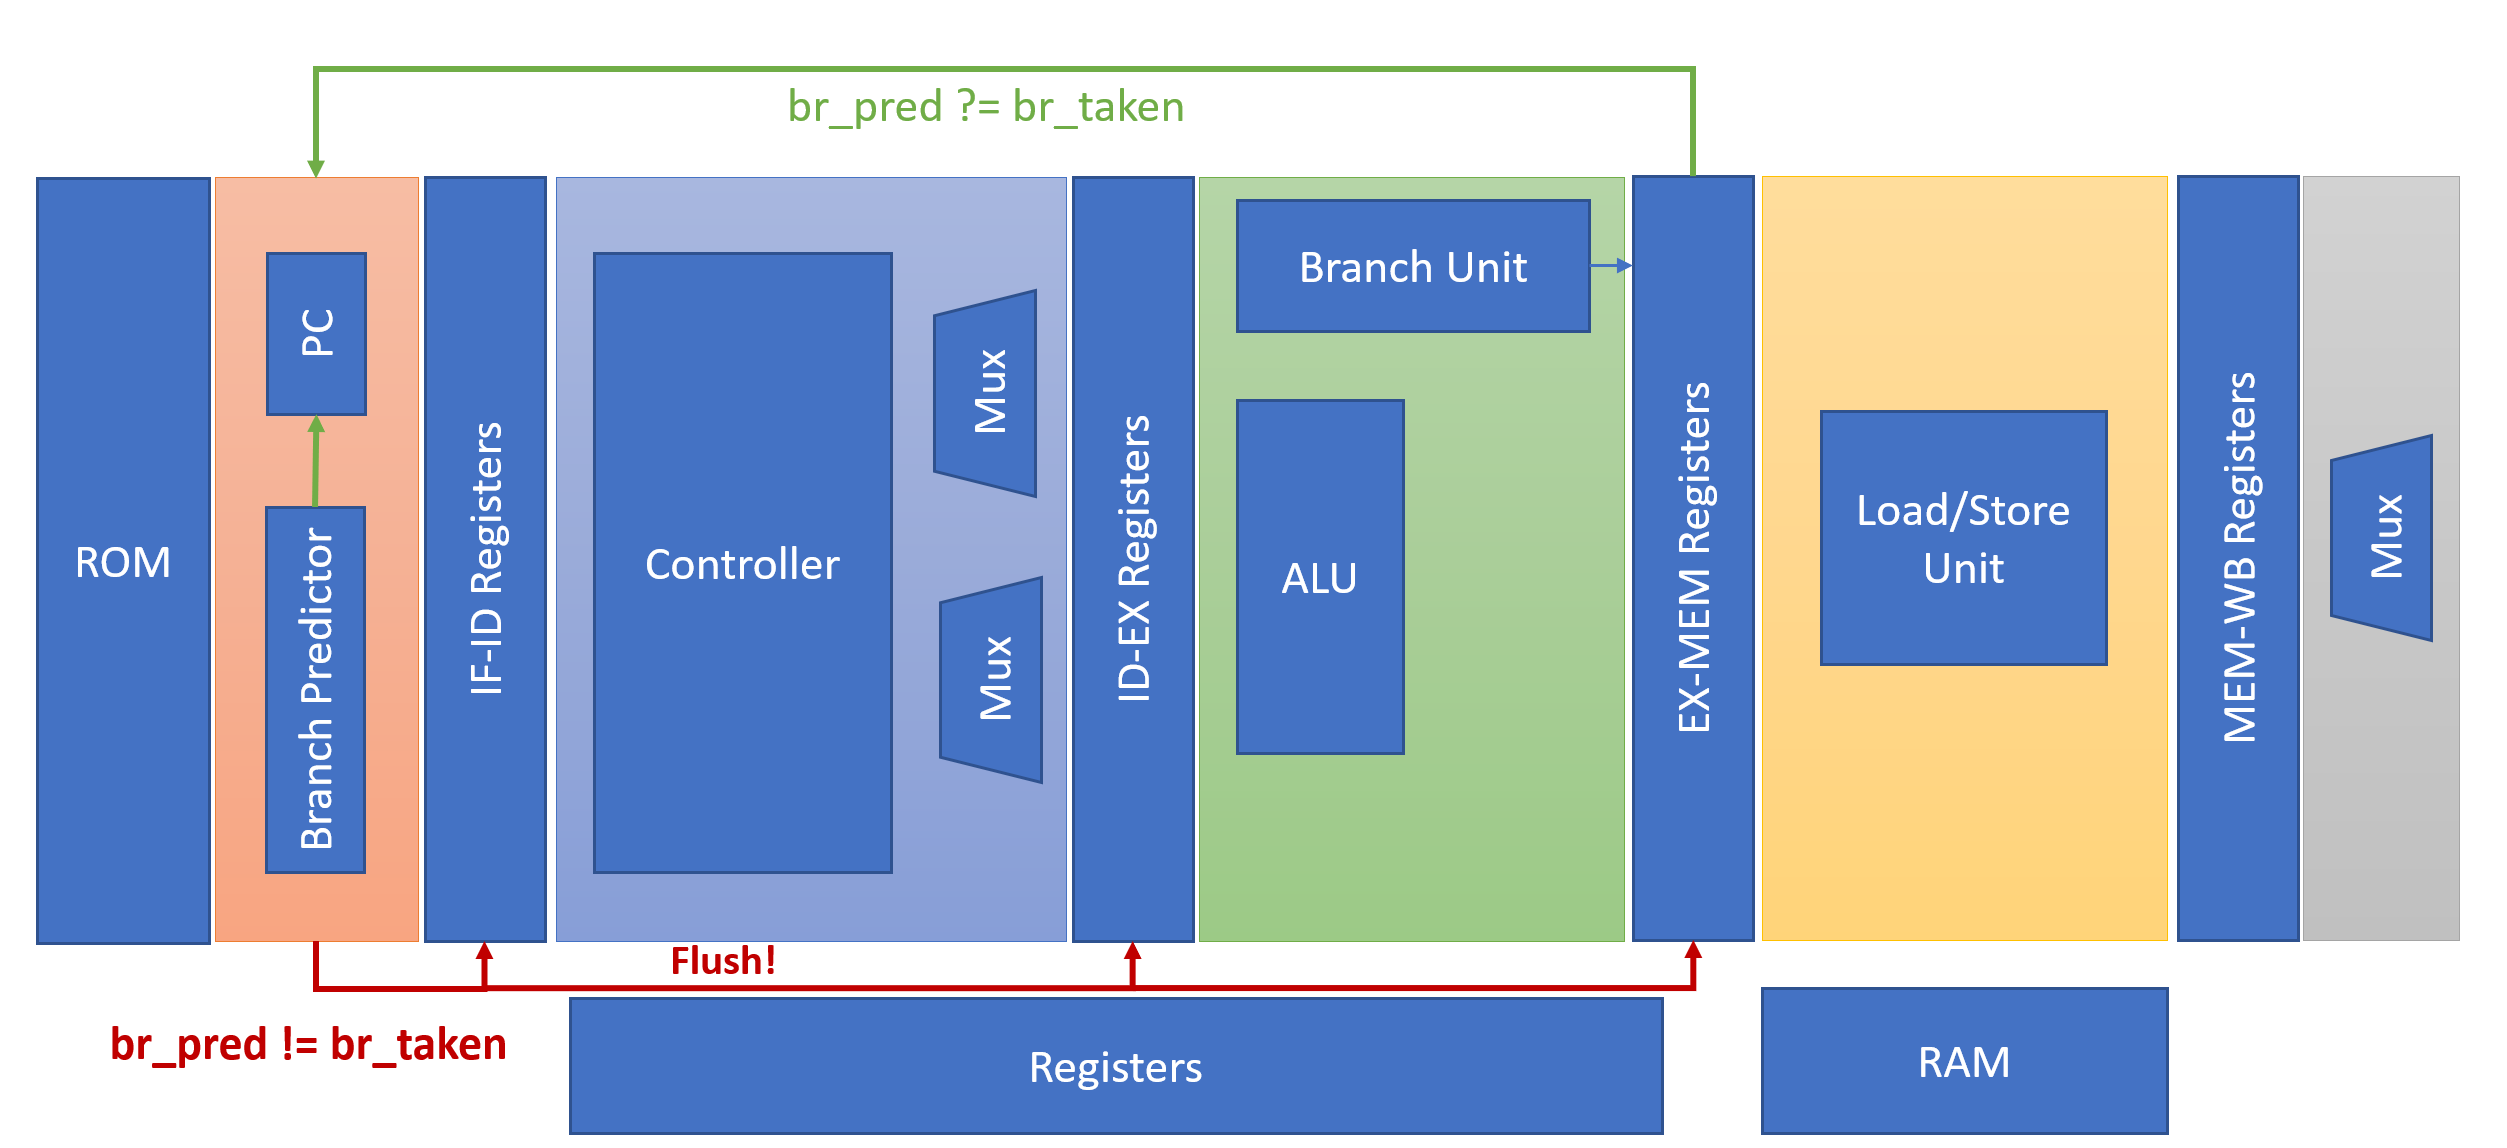
\includegraphics[width=1\textwidth]{design/pipelined/images/pipelined_design_predictor.png}
    \caption{Pipelined CPU design with branch predictor}
    \label{fig:pipelined_cpu_design_predictor}
\end{figure} 

Now we can see the full simplified representation of the pipelined CPU design. 
\begin{figure}[H]
    \centering
    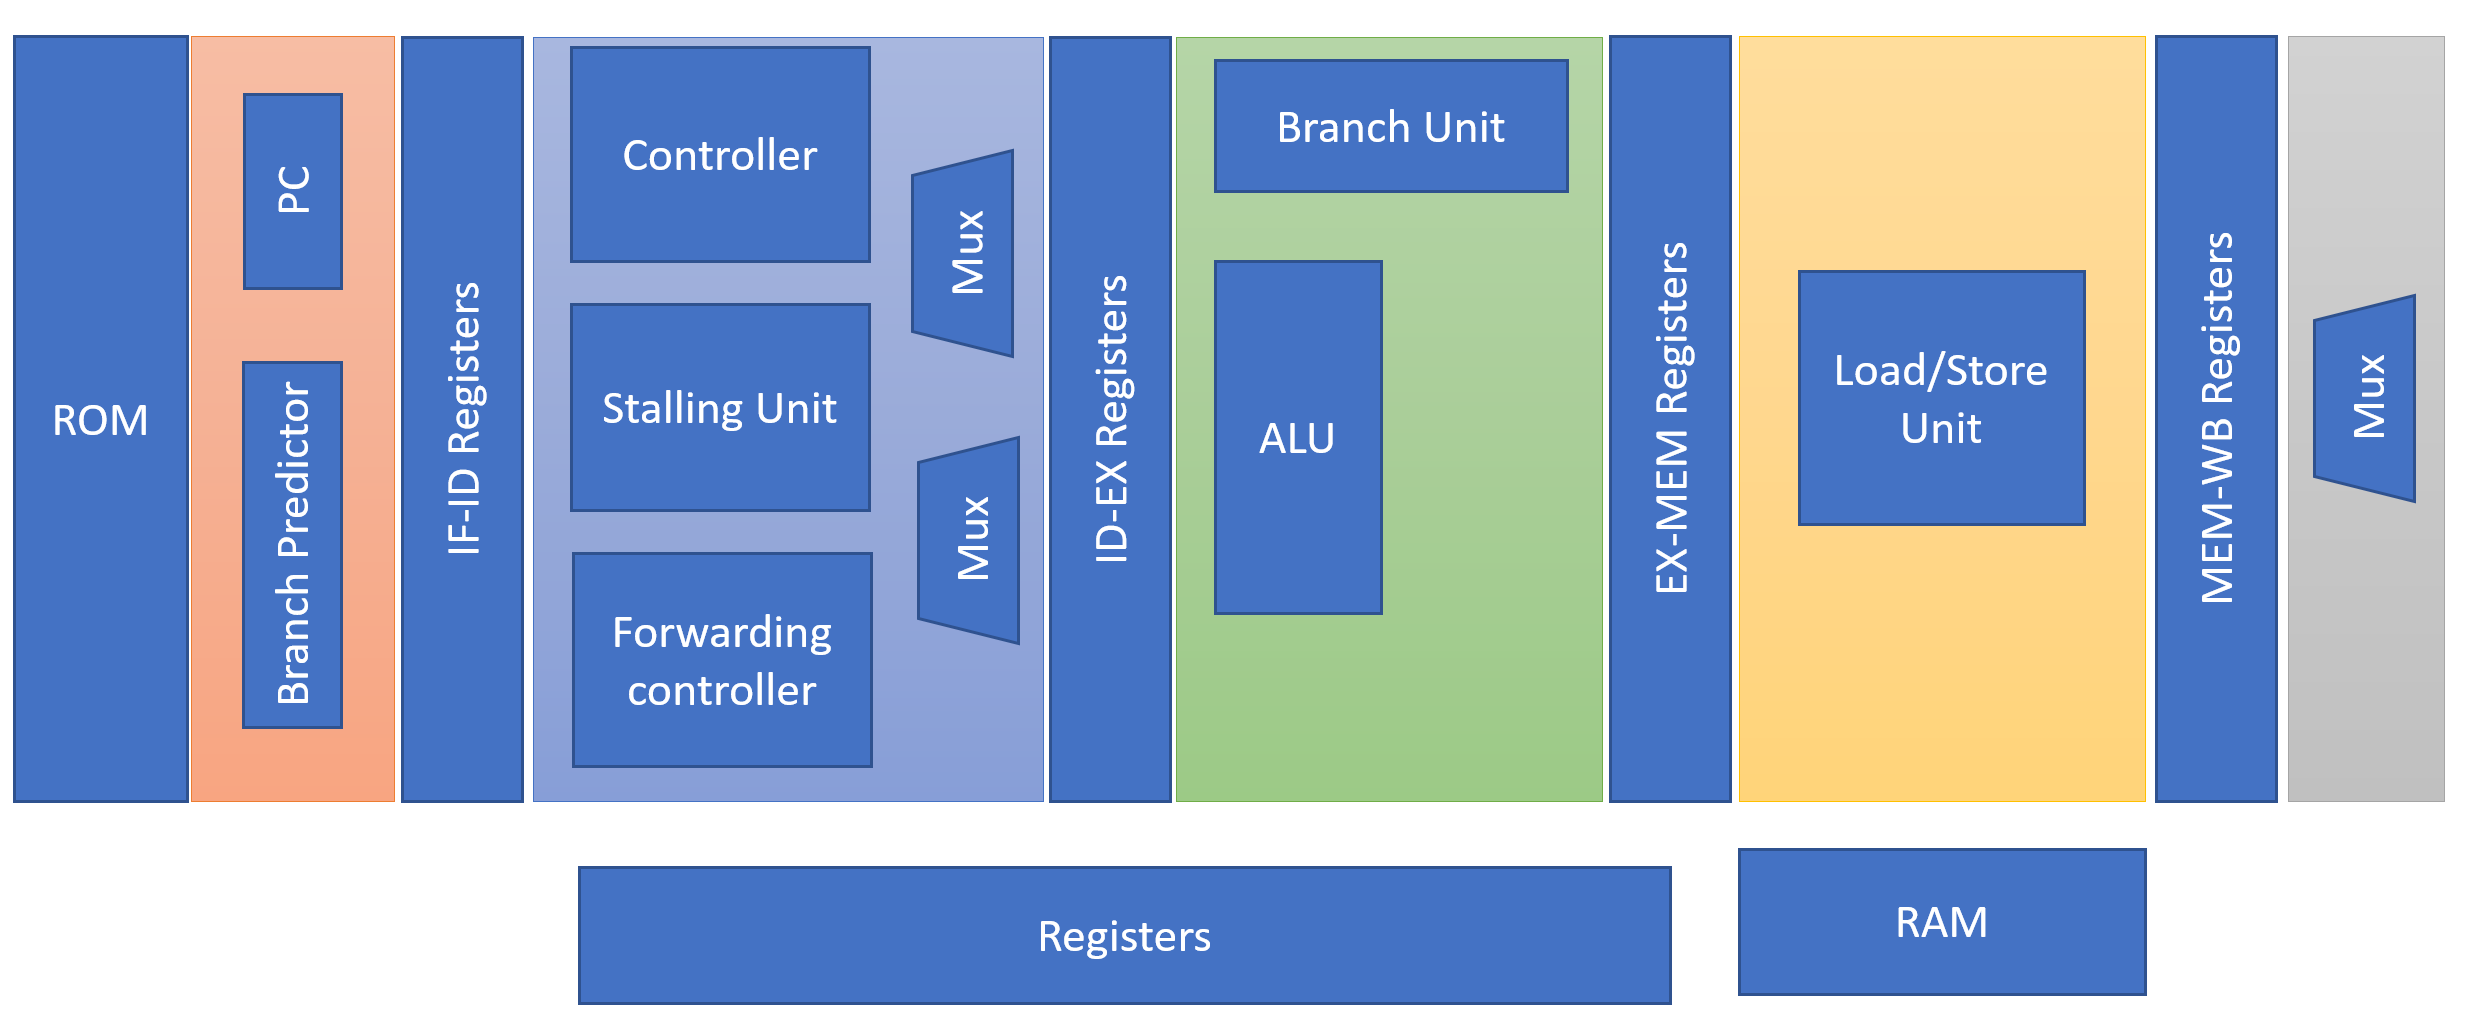
\includegraphics[width=1\textwidth]{design/pipelined/images/pipelined_design_full.png}
    \caption{Pipelined CPU simplified design with forwarding paths and branch predictor}
    \label{fig:pipelined_cpu_design_full}
\end{figure}

A more detailed version with all the different signals and how they are connected is available in the appendix \ref{appendix:pipelined_design} and
also as a diagram inside the project \texttt{diagrams} folder that can be opened \href{https://app.diagrams.net/}{here}. \\

Now that we have a better understanding of the overall design, I can go into more detail about each different stage and the modules inside of them.

\subsubsection{IF Stage}
\subsection{PC}

\begin{figure}[H]
\centering
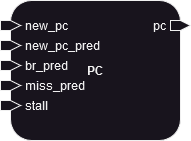
\includegraphics[width=0.5\textwidth]{../diagrams/fetch/pc.png}
\caption{Diagram of the PC}
\label{fig:PC}
\end{figure}

The PC is responsible for computing the next PC. It uses the different input signals to know which PC to compute.
for example, if it is a branch, the branch predictor will tell him what to do, and if the branch predictor is wrong
it will be updated accordingly. If it is a more classic instruction such as an ADD, it will simply increment the PC by 4
etc. \\

Signals:
\begin{enumerate}
    \item Input: $new\_pc$, This signal represent the next PC given by the branch unit in the EX stage.
    \item Input: $new\_pc\_pred$, This signal represent the next PC given by the branch predictor.
    \item Input: $br\_pred$, This signal is representing the state of the prediction made by the branch predictor in the EX stage.
    \item Input: $miss\_pred$, This signal is representing if there is a miss prediction or not.
    \item Input: $stall$, This signal is representing if the pipeline is stalled or not due to a data dependency in the ID stage.
    \item Output: $pc$, This signal is representing the current PC.
\end{enumerate}
\subsection{Branch Predictor}

\begin{figure}[H]
\centering
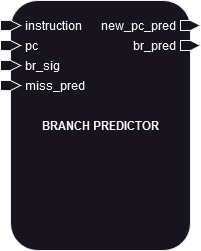
\includegraphics[width=0.5\textwidth]{../diagrams/fetch/br_predictor.png}
\caption{Diagram of the Branch Predictor}
\label{fig:br_predictor}
\end{figure}

The branch predictor as its name suggests is responsible for predicting if the branch will be taken or not. The algorithm that 
is being used is the two-level adaptive branch predictor, which I will not describe in detail but reuse the idea of a 
2-bit saturating counter but apply a bit of the notion of locality and pattern recognition. Of course, the algorithm
could be improved or replaced by any other algorithm and it is up to the user to do it if he wants to.
It works at the beginning by doing a simple matching on the current instruction to see if it is a branch instruction.
If that's the case we look if it is a conditional branch or not, if it is not we simply predict that the branch will be taken for 
the JAL instruction, but the JALR one will be always predicted as not taken for data dependency reasons. If it is a conditional branch
we simply use the algorithm described above to predict if the branch will be taken or not. The algorithm updates the prediction depending 
on the actual result of the branch that is represented by the $miss\_pred$ signal. If the prediction is taken, we compute the next PC \\

Signals:
\begin{enumerate}[label={\textbullet}]
    \item Input: $instruction$, This signal is representing the current instruction that is being fetched.
    \item Input: $pc$, This signal is representing the current PC.
    \item Input: $br\_sig$ This signal is representing the state of the current instruction in the EX stage. It is used to know if the instruction is a branch or not.
    such that it updates only the algorithm when it is a branch instruction.
    \item Input: $miss\_pred$, This signal is representing the state of the prediction made by the branch predictor in the EX stage.
    \item Output: $new\_pc\_pred$, This signal is representing the next PC that will be used if the prediction is taken.
    \item Output: $br\_pred$, This signal is indicating if the branch is predicted as taken or not.
\end{enumerate}


\subsubsection{ID Stage}
\subsection{Controller}

\begin{figure}[H]
\centering
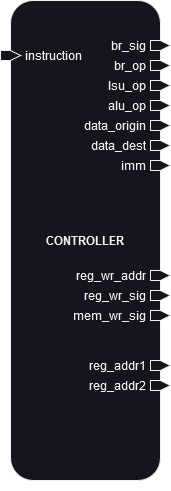
\includegraphics[width=0.35\textwidth]{../diagrams/decode/controller.png}
\caption{Diagram of the Controller}
\label{fig:controller}
\end{figure}

The controller is the main module of the ID stage. It is responsible for decoding the current instruction which is the action
of extracting the different fields of the instruction and forwarding them to the next stage. For more information about the different
types of instruction and how the data is encoded in the instruction, please refer to the RISC-V manual~\cite{riscv_manual}. \\

Signals:
\begin{enumerate}
    \item Input: $instruction$, This signal is representing the current instruction that is being decoded.
    \item Output: $br\_sig$, This signal is representing the state of the current instruction. 
    It is used to know if the instruction is a branch or not.
    \item Output: $br\_op$, This signal is representing the type of branch that is being executed.
    \item Output: $lsu_op$, This signal is representing the type of load or store that is being executed.
    \item Output: $alu\_op$, This signal is representing the type of ALU operation that is being executed.
    \item Output: $data\_origin$, This signal is representing the origin of the data that is being used by the ALU.
    That could be the registers, or one register and an immediate or one register and the PC.
    \item Output: $data\_dest$, This signal will be useful in the write-back stage to know which data to write back,
    so either the ALU result or the data from the memory or the next PC (so the PC+4).
    \item Output: $imm$, This signal is representing the immediate value that is being used by the ALU.
    \item Output: $reg\_wr\_addr$, This signal is representing the register address that will be written back.
    \item Output: $reg\_wr\_sig$, This signal is representing if we want to write to the register file or not.
    \item Output: $mem\_wr\_sig$, This signal is representing if we want to write to the memory or not.
    \item Output: $reg\_addr1$, This signal is representing the first register address that has been extracted from the instruction.
    \item Output: $reg\_addr2$, This signal is representing the second register address that has been extracted from the instruction.
\end{enumerate}
\subsection{Forward Controller}

\begin{figure}[H]
\centering
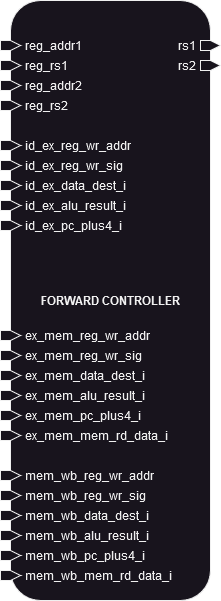
\includegraphics[width=0.35\textwidth]{../diagrams/decode/forward_controller.png}
\caption{Diagram of the Forward Controller}
\label{fig:forward_controller}
\end{figure}

The forward controller is a module that is used to control what are the values used as rs1 and rs2 in the ALU. 
For example, if you have a data dependency between two instructions, the first one is a load and the second one is an add,
you need to forward the result of the load to the ALU. This module is responsible for that and instead of using the value of the register file,
it will use the value that is being forwarded. \\

Signals:
\begin{enumerate}[label={\textbullet}]
    \item Input: $reg_addr1$, This signal is representing the first register address that is being used by the current instruction.
    \item Input: $reg_rs1$, This signal is representing the value of the first register that is being used by the current instruction.
    \item Input: $reg_addr2$, This signal is representing the second register address that is being used by the current instruction.
    \item Input: $reg_rs2$, This signal is representing the value of the second register that is being used by the current instruction.
    \item Input: $id\_ex\_reg\_wr\_addr$, This signal is representing the register address that is being written by the previous instruction.
    \item Input: $id\_ex\_reg\_wr\_sig$, This signal is representing if the previous instruction is written to the register file or not.
    \item Input: $id\_ex\_data\_dest$, This signal is representing the origin of the data that is being used by the ALU in the previous instruction.
    \item Input: $id\_ex\_alu\_result$, This signal is representing the result of the ALU in the previous instruction.
    \item Input: $id\_ex\_pc\_plus4$, This signal is representing the pc plus 4 of the previous instruction.
    \item Input: $ex\_mem\_reg\_wr\_addr$, This signal is representing the register address that is being written by the previous instruction.
    \item Input: $ex\_mem\_reg\_wr\_sig$, This signal is representing if the previous instruction is written to the register file or not.
    \item Input: $ex\_mem\_data\_dest$, This signal is representing the origin of the data that is being used by the ALU in the previous instruction.
    \item Input: $ex\_mem\_alu\_result$, This signal is representing the result of the ALU in the previous instruction.
    \item Input: $ex\_mem\_pc\_plus4$, This signal is representing the pc plus 4 of the previous instruction.
    \item Input: $ex\_mem\_mem\_rd\_data$, This signal is representing the data that is being read from the memory in the previous instruction.
    \item Input: $mem\_wb\_reg\_wr\_addr$, This signal is representing the register address that is being written by the previous instruction.
    \item Input: $mem\_wb\_reg\_wr\_sig$, This signal is representing if the previous instruction is written to the register file or not.
    \item Input: $mem\_wb\_data\_dest$, This signal is representing the origin of the data that is being used by the ALU in the previous instruction.
    \item Input: $mem\_wb\_alu\_result$, This signal is representing the result of the ALU in the previous instruction.
    \item Input: $mem\_wb\_pc\_plus4$, This signal is representing the pc plus 4 of the previous instruction.
    \item Input: $mem\_wb\_mem\_rd\_data$, This signal is representing the data that is being read from the memory in the previous instruction.
    \item Output: $rs1$, This signal is representing the value that should be used as rs1 in the ALU.
    \item Output: $rs2$, This signal is representing the value that should be used as rs2 in the ALU.
\end{enumerate}
\paragraph{Stall Unit}

\begin{figure}[H]
    \centering
    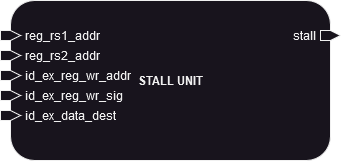
\includegraphics[width=0.5\textwidth]{design/pipelined/decode/images/stall_unit.png}
    \caption{Diagram of the Stall Unit}
    \label{fig:stall_unit}
\end{figure}

The stall unit is a small module that is used to stall the pipeline when a data dependency that cannot be resolved by forwarding is detected
which should only happen if we use the result of a load instruction in the next instruction. It is simply comparing the register addresses of the
current instruction with the register that is being written by the previous instruction. If there is a match, it looks what is the operation that is
being executed by the current instruction and if it is a load, it will stall the pipeline. \\

Signals:
\begin{enumerate}[label={\textbullet}]
    \item Input: $reg\_rs1\_addr$, This signal is representing the first register address that is being used by the current instruction.
    \item Input: $reg\_rs2\_addr$, This signal is representing the second register address that is being used by the current instruction.
    \item Input: $id\_ex\_reg\_wr\_addr$, This signal is representing the register address that is being written by the previous instruction.
    \item Input: $id\_ex\_reg\_wr\_sig$, This signal is representing if the previous instruction is written to the register file or not.
    It is used to differentiate between a load and a store.
    \item Input: $id\_ex\_data\_dest$, This signal is representing the origin of the data that is being used by the ALU in the previous instruction.
    In this case only if the previous instruction has a data dest of MEM then we need to stall the pipeline.
    \item Output: $stall$, This signal is representing if we need to stall the pipeline or not.
\end{enumerate}
\paragraph{Mux}

\begin{figure}[H]
    \centering
    
\includegraphics[width=0.20\textwidth]{design/pipelined/decode/images/mux2.png}
    \caption{Diagram of the 2 entries Mux}
    \label{fig:mux2}
\end{figure}

The mux is a small module that is used to select between the two inputs that it has. It is used 2 times in this module, for selecting between
$rs1$ and $PC$ and for selecting between $rs2$ and $imm$. Sorry, I haven't used the standard shape of a MUX but I haven't found one on the 
website I'm using to draw the different diagrams. \\

Signals:
\begin{enumerate}[label={\textbullet}]
    \item Input: $a$, This signal is representing the first input of the mux.
    \item Input: $b$, This signal is representing the second input of the mux.
    \item Input: $sel$, This signal is representing the select signal of the mux.
    \item Output: $out$, This signal is representing the output of the mux.
\end{enumerate}

\subsubsection{EX Stage}
\subsection{ALU}

\begin{figure}[H]
\centering
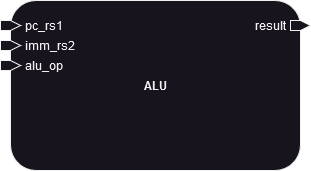
\includegraphics[width=0.75\textwidth]{../diagrams/execute/alu.png}
\caption{Diagram of the ALU}
\label{fig:alu}
\end{figure}

The ALU is a module that is responsible for executing the arithmetic and logic operations. So every mathematical operation is done in this module.

Signals:
\begin{enumerate}[label={\textbullet}]
    \item Input: $a$, This signal is representing the first input of the ALU.
    \item Input: $b$, This signal is representing the second input of the ALU.
    \item Input: $op$, This signal is representing the operation that the ALU will execute.
    \item Output: $out$, This signal is representing the output of the ALU.
\end{enumerate}
\subsection{Branch Unit}

\begin{figure}[H]
\centering
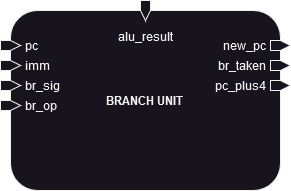
\includegraphics[width=0.5\textwidth]{../diagrams/execute/br_unit.png}
\caption{Diagram of the Branch Unit}
\label{fig:br_unit}
\end{figure}

The Branch Unit is a module that is responsible for computing the next PC. It is used in the EX stage. It uses the result of the ALU
for conditional branching to know if the branch should be taken or not.

Signals:
\begin{enumerate}[label={\textbullet}]
    \item Input: $alu\_result$, This signal is representing the result of the ALU. Used for conditional branching.
    \item Input: $pc$, This signal is representing the current PC.
    \item Input: $imm$, This signal is representing the immediate value of the instruction. It is used as an offset for the branch.
    \item Input: $branch\_sig$, This signal mark if the instruction is a branch or not.
    \item Input: $br\_op$, This signal is representing the branch operation like for example BEQ, BNE etc.
    \item Output: $new\_pc$, This signal is representing the new PC computed by the branch unit.
    \item Output: $pc\_plus\_four$, This signal is representing the PC + 4. Used to save the value of the next instruction 
    to come back at it after a branch occurred.
    \item Output: $br\_taken$, This signal is representing if the branch is taken or not. Used in the IF stage to compare 
    to the branch predictor and know if the pipeline needs to be flushed or not.
\end{enumerate}

\subsubsection{MEM Stage}
\subsection{Load Store Unit}

\begin{figure}[H]
    \centering
    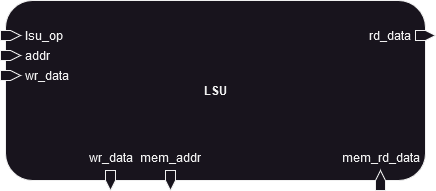
\includegraphics[width=0.5\textwidth]{../diagrams/memory/lsu.png}
    \caption{Load Store Unit}
    \label{fig:lsu}
\end{figure}

The LSU is a module that is responsible for memory access. It will manage the different READ and WRITE to the memory and for example
mask the data you want to read or write according to the given instruction.

Signals:
\begin{enumerate}[label={\textbullet}]
    \item Input: $lsu\_op$, This signal is representing the type of memory access you want to perform.
    \item Input: $addr$, This signal is representing the address of the memory you want to access.
    \item Input: $wr\_data$, This signal is representing the data you want to write to the memory.
    \item Input: $mem\_rd\_data$, This signal is representing the value that has been read from the memory.
    \item Output: $wr\_data$, This signal is representing the value that should be written to the memory and correctly
    masked according to the given instruction.
    \item Output: $mem\_addr$, This signal is representing the address you want to write or read to the memory.
    \item Output: $rd\_data$, This signal represents the value that has been read from the memory and correctly 
    masked according to the given instruction.
\end{enumerate}

\subsubsection{WB Stage}
\paragraph{Mux}

\begin{figure}[H]
    \centering
    
\includegraphics[width=0.20\textwidth]{design/pipelined/decode/images/mux2.png}
    \caption{Diagram of the 2 entries Mux}
    \label{fig:mux2}
\end{figure}

The mux is a small module that is used to select between the two inputs that it has. It is used 2 times in this module, for selecting between
$rs1$ and $PC$ and for selecting between $rs2$ and $imm$. Sorry, I haven't used the standard shape of a MUX but I haven't found one on the 
website I'm using to draw the different diagrams. \\

Signals:
\begin{enumerate}[label={\textbullet}]
    \item Input: $a$, This signal is representing the first input of the mux.
    \item Input: $b$, This signal is representing the second input of the mux.
    \item Input: $sel$, This signal is representing the select signal of the mux.
    \item Output: $out$, This signal is representing the output of the mux.
\end{enumerate}

\subsubsection{Pipeline Registers}
\begin{figure}[H]
    \centering
    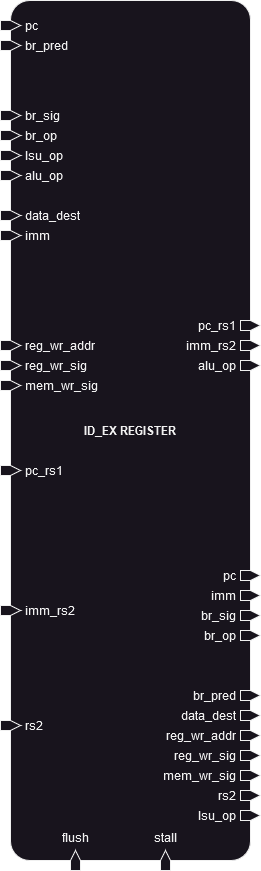
\includegraphics[width=0.35\textwidth]{design/pipelined/pipeline/images/pipeline.png}
    \caption{ID-EX Pipeline register example}
    \label{fig:pipeline}
\end{figure}

I will not explain the 4 different pipeline register stages in detail, and I will mainly describe as an example the 
pipeline between the ID Stage and the Ex Stage. The role of a pipeline register is to store the data that will be
passed to the next stage at each clock cycle such that you can increase throughput by increasing the clock frequency since 
you've divided the overall work in smaller chunks so you can do it in less time (theoretically).
What is also interesting here is the $stall$ and $flush$ signals. The first one is used to stop updating the pipeline when 
a data dependency is encountered. The second one is used when the branch predictor did a bad guess. In this case we need to 
flush the register that has incorrect instructions stored in them and instead just fill them with something similar to a NOP 
instruction.

\subsubsection{ROM, RAM and Register File}
\subsection{ROM}

\begin{figure}[H]
    \centering
    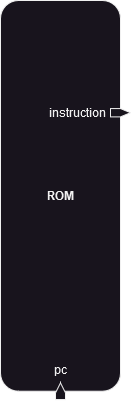
\includegraphics[width=0.35\textwidth]{../diagrams/rom_ram_reg/rom.png}
    \caption{ROM}
    \label{fig:rom}
\end{figure}

The ROM is responsible for storing the program that is being executed by the processor. As its name indicate, it is 
a read-only memory and for the moment it is capable of storing up-to 1024 instructions.

Signals:
\begin{enumerate}[label={\textbullet}]
    \item Input: $pc$, This signal gives the address that needs to be read in the memory.
    \item Output: $instruction$, This signal is representing the instruction that has been read from the ROM.
\end{enumerate}
\paragraph{RAM}

\begin{figure}[H]
    \centering
    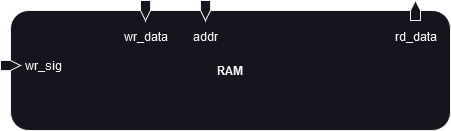
\includegraphics[width=0.5\textwidth]{design/pipelined/rom_ram_reg/images/ram.png}
    \caption{RAM}
    \label{fig:ram}
\end{figure}

The RAM is the main memory of the CPU, it can be used to store and read values. In this project, the RAM is also 1024 words long
and each word is 32 bits long.

Signals:
\begin{enumerate}[label={\textbullet}]
    \item Input: $addr$, This signal gives the address that needs to be read or written in the memory.
    \item Input: $wr\_sig$, This signal indicates if the given address need to be written or read
    \item Input: $wr\_data$, This signal gives the data that needs to be written in the memory.
    \item Output: $rd\_data$, This signal is representing the data that has been read from the RAM.
\end{enumerate}
\paragraph{Register File}

\begin{figure}[H]
    \centering
    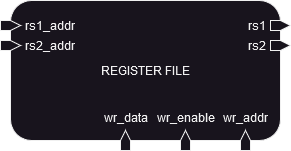
\includegraphics[width=0.5\textwidth]{design/pipelined/rom_ram_reg/images/register_file.png}
    \caption{Register File}
    \label{fig:register_file}
\end{figure}

The register file is a one-cycle really small memory. The RV32I standard requires 32 registers, each 32 bits long. Only the first (zero) register
has a given value of 0, the other can be used at will but as with any other architecture there are some standards for what a register is being used 
for.

Signals:
\begin{enumerate}[label={\textbullet}]
    \item Input: $rs1\_addr$, This signal gives the address of the first register that needs to be read.
    \item Input: $rs2\_addr$, This signal gives the address of the second register that needs to be read.
    \item Input: $wr\_addr$, This signal gives the address of the register that needs to be written.
    \item Input: $wr\_data$, This signal gives the data that needs to be written in the memory.
    \item Input: $wr\_enable$, This signal indicates whether the register should be written with the $wr\_data$ value.
    \item Output: $rs1$, This signal gives the value read at address $rs1\_addr$.
    \item Output: $rs2$, This signal gives the value read at address $rs2\_addr$.
\end{enumerate}








